\input templates/header
\title[ASD - Problemi \NP-completi]{\textbf{Algoritmi e Strutture Dati}\\[12pt]Problemi intrattabili\\Teoria dell'NP-completezza}


\usepackage{xcolor}
\usepackage{colortbl}

\newcommand{\PTIME}{\mbox{\sc $\mathbb{P}$}}
\renewcommand{\NP}{\mbox{$\mathbb{NP}$}}
\newcommand{\TIME}{\mbox{$\mathbb{TIME}$}}
\newcommand{\EXPTIME}{\mbox{$\mathbb{EXPTIME}$}}
\newcommand{\SPACE}{\mbox{$\mathbb{SPACE}$}}
\newcommand{\PSPACE}{\mbox{$\mathbb{PSPACE}$}}

\newcommand{\R}[1]{\textcolor{red}{#1}}
\newcommand{\B}[1]{\textcolor{blue}{#1}}

\renewcommand{\arraystretch}{1.4}
\graphicspath{{figs/18/}}


\begin{document}

%-------------------------------------------------------------------------
\FrameTitle{}

%-------------------------------------------------------------------------
\FrameContent



%%%%%%%%%%%%%%%%%%%%%%%%%%%%%%%%%%%%%%%%%%%%%%%%%%%%%%%%%%%%%%%%%%%%%%%%%%
\section{Introduzione}

%-------------------------------------------------------------------------
\begin{frame}{Introduzione}

\vspace{-9pt}
\BB{Con l'eccezione della sezione su backtrack, finora abbiamo considerato solo 
problemi con soluzioni in tempo polinomoniale}
\BIL
\item  Il tempo di esecuzione è $O(n^k)$ per qualche $k$
\EIL

\medskip
\BB{Sono gli unici problemi interessanti?}
\BIL
\item Esistono problemi che per essere risolti hanno
  bisogno di un tempo almeno esponenziale (\EXPTIME)
    \BI
    \item Valutare una posizione di scacchi, dama, go; 
    \item Risolvere il problema delle Torri di Hanoi
    \EI
\item Esistono problemi per i quali non esiste alcuna soluzione
  \BI
  \item Halting problem
  \EI
\EIL

\end{frame}

%-------------------------------------------------------------------------
\begin{frame}{Introduzione}

\vspace{-9pt}
\begin{myboxtitle}[Obiettivo della lezione]
\BIL
\item Discuteremo di un classe di problemi per cui non è chiaro se esiste
un algoritmo polinomiale oppure no
\item Questi problemi sono tutti sulla stessa barca: 
  possono essere tutti risolti in tempo polinomiale, oppure nessuno
\item Questa classe contiene tantissimi problemi interessanti!
\EIL
\end{myboxtitle}

\begin{myboxtitle}[Millenium Prize Problems, Clay Institute]
\BI
\item Premio istituito nel 2000
\item Sette problemi matematici aperti
\item 1M\euro\ per chi li risolve
\item Ad oggi, un solo problema risolto (Congettura di Poincarè)
\EI
\end{myboxtitle}

\end{frame}


%-------------------------------------------------------------------------
\begin{frame}{Alcune definizioni}

\vspace{-9pt}
\begin{myboxtitle}[Problema astratto]
Una \alert{problema astratto} è una relazione binaria $R \subseteq I \times S$
tra un insieme $I$ di istanze del problema e un insieme $S$ di
soluzioni
\end{myboxtitle}

\begin{myboxtitle}[Esempio -- \textsc{shortest-path}]
\BIL
\item Un'istanza è una quadrupla $(V,E,u,v)$
\item Una soluzione è una sequenza ordinata di vertici $v_1 \ldots v_k$
\item Nota: possono esistere più soluzioni associate alla stessa istanza
\EIL
\end{myboxtitle}

\end{frame}


%-------------------------------------------------------------------------
\begin{frame}{Tipologia di problemi}

\small
\vspace{-15pt}
\begin{columns}[T]
\column{0.49\textwidth}
\begin{myboxtitle}[Problemi di \alert{ottimizzazione}]
\BI
\item Data un'istanza, trovare la "migliore" soluzione secondo criteri specifici
\item \alert{\textsc{shortest-path} (Opt.)}:
Dati un grafo $G$ e due nodi $u, v$,
trovare il cammino più breve fra essi
\EI
\end{myboxtitle}
\column{0.49\textwidth}
\begin{myboxtitle}[Problemi di \alert{ricerca}]
\BI
\item Data un'istanza, trovare una possibile soluzione fra quelle esistenti
\item \alert{\textsc{path}}: Dati un grafo $G$ e due nodi $u, v$, trovare un
cammino fra essi
\EI
\end{myboxtitle}
\end{columns}

\begin{myboxtitle}[Problemi di \alert{decisione}]
\BI
\item Data un'istanza, verificare se soddisfa o meno una data proprietà\\
La relazione $R$ è una funzione $R: I \rightarrow \{ 0, 1 \}$ 
\item \alert{\textsc{shortest-path} (Dec.)}: Dati un grafo $G$, due nodi $u,v$  e un valore $k$, esiste un cammino tra $u$ e $v$ di lunghezza minore o uguale a $k$?
\EI
\end{myboxtitle}


\end{frame}

%-------------------------------------------------------------------------
\begin{frame}{Equivalenza problemi di ottimizzazione / decisione}

\vspace{-9pt}
\BB{Ragioneremo in termini di problemi di decisione}
\BIL
\item La versione decisionale è più semplice da trattare matematicamente
\item Se posso risolvere efficientemente la versione di ottimizzazione
$\Rightarrow$ \\ posso risolvere efficientemente la versione di decisione 
\item \alert{Se \emph{non} posso risolvere efficientemente la versione di decisione
$\Rightarrow$ \\ \emph{non} posso risolvere efficientemente la versione di ottimizzazione}
\EIL

\begin{myboxtitle}[Esempio -- Shortest path]
\BIL
\item Se conosco il cammino più breve, posso rispondere alla domanda decisionale
per qualunque valore di $k$
\EIL
\end{myboxtitle}


\end{frame}

\section{Riduzioni}

%-------------------------------------------------------------------------
\begin{frame}{Riduzione polinomiale}

\vspace{-9pt}
\begin{myboxtitle}[Riduzione polinomiale]
Dati due problemi decisionali $R_1 \subseteq I_1 \times \{ 0,1 \}$ e
$R_2 \subseteq I_2 \times \{ 0,1 \}$, $R_1$ è \alert{riducibile polinomialmente} a $R_2$ (\alert{$R_1 \leq_p R_2$}) se esiste una funzione
$f: I_1 \rightarrow I_2$ con le seguenti proprietà:
\BI
\item $f$ è calcolabile in tempo polinomiale;
\item per ogni istanza $x$ del problema $R_1$ e
  ogni soluzione $s \in \{ 0,1 \}$, 
  $(x,s) \in R_1$ $\Leftrightarrow$ $(f(x),s) \in R_2$.
\EI
\end{myboxtitle}

\IG{0.9}{riduzione.pdf}

\end{frame}

%-------------------------------------------------------------------------
\begin{frame}{Colorazione di grafi}

\vspace{-9pt}
\begin{myboxtitle}[Colorazione di grafi (\textsc{graph-coloring})]
Dati un grafo non orientato $G=(V,E)$ e un insieme di colori $C$, una \alert{colorazione} dei vertici è un assegnamento  $f: V \rightarrow C$
\BI
\item che ``colora'' ogni nodo con uno dei valori in $C$, 
\item tale per cui nessuna coppia di nodi adiacenti ha lo stesso colore.
\EI
\end{myboxtitle}

\vspace{-12pt}
\TwoCols{
\begin{center}
\IG{0.54}{coloring.pdf}
\end{center}
}{
\begin{center}
\IG{0.40}{4colors.pdf}
\end{center}
}
\tiny
\url{https://it.wikipedia.org/wiki/Colorazione_dei_grafi\#/media/File:Petersen_graph_3-coloring.svg}
\url{https://en.wikipedia.org/wiki/Four_color_theorem\#/media/File:Four_Colour_Map_Example.svg}
\end{frame}

%-------------------------------------------------------------------------
\begin{frame}{Colorazione di grafi}

\vspace{-9pt}
\begin{myboxtitle}[Colorazione, ottimizzazione]
Dato un grafo non orientato $G=(V,E)$, restituire la colorazione che richiede il minimo numero di colori
\end{myboxtitle}

\begin{myboxtitle}[Colorazione, decisionale]
Dato un grafo non orientato $G=(V,E)$ e un valore $k$, determinare se esiste
una colorazione di $G$ con $k$ colori
\end{myboxtitle}

\end{frame}

%-------------------------------------------------------------------------
\begin{frame}{Sudoku}

\vspace{-9pt}
\begin{myboxtitle}[\textsc{sudoku}]
Il problema generale del \alert{Sudoku} richiede di inserire dei numeri
fra $1$ e $n^2$ in una matrice di $n^2 \times n^2$ elementi 
suddivisa in $n \times n$ sottomatrici di dimensione $n \times n$, 
in modo tale che nessun  numero compaia più di una volta in ogni 
riga, colonna e sottomatrice
\end{myboxtitle}

\begin{myboxtitle}[\textsc{sudoku}, decisionale]
Data una matrice $n^2 \times n^2$ elementi, determinare se esiste un modo per assegnare i numeri in modo da rispettare le regole del Sudoku
\end{myboxtitle}

\begin{myboxtitle}[\textsc{sudoku-precolored}, decisionale]
Data una matrice $n^2 \times n^2$ elementi con alcuni numeri già presenti nella matrice, determinare se esiste un modo per assegnare i numeri in modo da rispettare le regole del Sudoku
\end{myboxtitle}

\end{frame}


%-------------------------------------------------------------------------
\begin{frame}{Riduzione da problema particolare a problema generale}

\small
\vspace{-17pt}
\begin{columns}[T]
\column{0.59\textwidth}
\begin{myboxtitle}[Riduzione in tempo polinomiale]
\noindent
$V=\{ (x,y) : 1 \leq x \leq n^2, 1 \leq y \leq n^2 \}$

\smallskip\noindent
$[(x,y), (x',y')] \in E \Leftrightarrow {}$
\BI
\item $x=x'$; oppure,
\item $y=y'$; oppure,
\item $(\lceil x/n \rceil = \lceil x'/n \rceil) \wedge (\lceil y/n \rceil = \lceil y'/n \rceil)$
\EI
\smallskip\noindent
$C = \{1, \ldots, n \}$.
\end{myboxtitle}

\vspace{-9pt}
\begin{center}
\IG{0.9}{sudoku.jpg}
\end{center}

\column{0.39\textwidth}
\begin{myboxtitle}[Riduzione]
$\textsc{sudoku} \leq_p {}$\\
$\textsc{graph-coloring}$

\smallskip
Se abbiamo una soluzione per la colorazione, allora abbiamo una soluzione algoritmica per il Sudoku
\end{myboxtitle}

\begin{myboxtitle}[Applicazioni]
\noindent
Assegnamento radio frequenze in un insieme di torri cellulari

\medskip\noindent
Allocazione degli esami universitari
\end{myboxtitle}

\end{columns}

\end{frame}


%-------------------------------------------------------------------------
\begin{frame}{Insieme indipendente}

\vspace{-9pt}
\begin{myboxtitle}[Insieme Indipendente (\textsc{independent-set})]
Sia dato un grafo non orientato $G=(V,E)$; un insieme
$S \subseteq V$ è un \alert{insieme indipendente} $\Leftrightarrow$ nessun arco unisce due nodi in $S$

\vspace{-3pt}
\[
\forall (x,y) \in E: x \not \in S \vee y \not \in S
\]
\end{myboxtitle}

\bigskip
\begin{overprint}
\onslide<1|handout:1>
\begin{center}
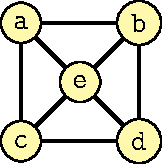
\includegraphics[width=0.3\textwidth,page=1]{independent.pdf}
\end{center}
\onslide<2|handout:2>
\begin{center}
\includegraphics[width=0.3\textwidth,page=2]{independent.pdf}
\end{center}
\end{overprint}

\end{frame}


%-------------------------------------------------------------------------
\begin{frame}{Insieme indipendente}

\vspace{-9pt}
\begin{myboxtitle}[\textsc{independent-set}, ottimizzazione]
Dato un grafo non orientato $G=(V,E)$, restituire il più grande insieme indipendente presente nel grafo
\end{myboxtitle}

\begin{myboxtitle}[\textsc{independent-set}, decisionale]
Dato un grafo non orientato $G=(V,E)$ e un valore $k$, determinare se esiste un insieme indipendente di dimensione almeno $k$
\end{myboxtitle}

\begin{myboxtitle}[Packing problem]
Questo è un esempio di \alert{packing problem}, un problema in cui si cerca
di selezionare il maggior numero di oggetti, la cui scelta è però soggetta
a vincoli di esclusione
\end{myboxtitle}

\end{frame}


%-------------------------------------------------------------------------
\begin{frame}{Copertura di vertici}


\vspace{-9pt}
\begin{myboxtitle}[Copertura di vertici (\textsc{vertex-cover})]
Dato un grafo non orientato $G=(V,E)$, un insieme
$S \subseteq V$ è una \alert{copertura di vertici} $\Leftrightarrow$ ogni arco ha almeno un  estremo in $S$

\vspace{-3pt}
\[
  \forall (x,y) \in E: x \in S \vee y \in S
\]
\end{myboxtitle}

\bigskip
\begin{overprint}
\onslide<1|handout:1>
\begin{center}
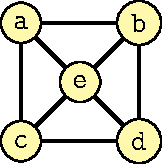
\includegraphics[width=0.3\textwidth,page=1]{cover.pdf}
\end{center}
\onslide<2|handout:2>
\begin{center}
\includegraphics[width=0.3\textwidth,page=2]{cover.pdf}
\end{center}
\end{overprint}

\end{frame}

%-------------------------------------------------------------------------
\begin{frame}{Copertura di vertici}

\vspace{-9pt}
\begin{myboxtitle}[\textsc{vertex-cover}, ottimizzazione]
Dato un grafo non orientato $G=(V,E)$, restituire la copertura dei vertici
di dimensione minima.
\end{myboxtitle}

\begin{myboxtitle}[\textsc{vertex-cover}, decisionale]
Dato un grafo non orientato $G=(V,E)$ e un valore $k$, determinare se
esiste una copertura di vertici di dimensione al massimo $k$
\end{myboxtitle}

\begin{myboxtitle}[Covering problem]
Questo è un esempio di \alert{covering problem}, un problema in cui si cerca
di ottenere il più piccolo insieme in grado di coprire un insieme 
arbitrario di oggetti con il più piccolo sottoinsieme di questi oggetti.
\end{myboxtitle}

\end{frame}

%-------------------------------------------------------------------------
\begin{frame}{Riduzione per problemi duali}

\vspace{-9pt}
\BB{$S \subseteq V$ è un independent set $\Rightarrow$ $V-S$ è un vertex cover}
Se $S$ è un insieme indipendente:
\BI
\item ogni arco $(x,y)$ non può avere entrambi gli estremi in $S$; 
\item quindi almeno uno dei due deve essere in $V-S$, \textsc{cvd}
\EI

\begin{center}
\includegraphics[width=0.6\textwidth,page=3]{independent.pdf}
\end{center}

\end{frame}

\begin{frame}{Riduzione per problemi duali}

\vspace{-9pt}
\BB{$V-S$ è un vertex cover $\Rightarrow$ $S \subseteq V$ è un independent set}
Supponiamo per assurdo che $S$ non sia un independent set:
\BI
\item allora esiste un arco $(x,y)$ che unisce due nodi in $S$
\item nessuno dei due estremi sta in $V-S$
\item questo implica che $V-S$ non è un vertex cover, assurdo
\EI

\begin{center}
\includegraphics[width=0.6\textwidth,page=3]{cover.pdf}
\end{center}

\end{frame}

%-------------------------------------------------------------------------
\begin{frame}{Riduzione per problemi duali}

\vspace{-9pt}
\BB{$\textsc{vertex-cover} \leq_p \textsc{independent-set}$\\ $\textsc{independent-set} \leq_p \textsc{vertex-cover}$}
Abbiamo quindi dimostrato che i due problemi sono equivalenti.

\end{frame}

%-------------------------------------------------------------------------
\begin{frame}{SAT}

\vspace{-9pt}
\begin{myboxtitle}[Formule booleane in forma normale congiuntiva]
Dato un insieme $V$ contenente $n$ \alert{variabili}
\BIL
\item un \alert{letterale} è una variabile $v$ oppure la sua negazione $\overline{v}$
\item una \alert{clausola} è una disgiunzione di letterali (letterali separati da \textbf{or})
\item una \alert{formula in forma normale congiuntiva} è una congiunzione di clausole (clausole separate da \textbf{and})
\EIL
\end{myboxtitle}

\begin{myboxtitle}[Esempio]
\[
  (x \vee \overline{y} \vee z) \wedge (\overline{x} \vee w) \wedge y
\]
\end{myboxtitle}

\end{frame}

%-------------------------------------------------------------------------
\begin{frame}{SAT}

\vspace{-9pt}
\begin{myboxtitle}[Soddisfacibilità di formule booleane (\textsc{SATisfiability})]
Data un'espressione in forma normale congiuntiva, il problema
della \alert{soddisfacibilità} consiste nel decidere se esiste una
assegnazione di valori di verità alle variabili che rende
l'espressione vera. 
\end{myboxtitle}

\begin{myboxtitle}[Esempio]
\[
  (x \vee \overline{y} \vee z) \wedge (\overline{x} \vee w) \wedge y
\]
\pause
\[
x = \TRUE, y = \TRUE, w = \TRUE, z = \TRUE \}
\]
\[
  (\TRUE \vee \FALSE \vee \TRUE) \wedge (\FALSE \vee \TRUE) \wedge \TRUE
\]
\end{myboxtitle}

\end{frame}

%-------------------------------------------------------------------------
\begin{frame}{3-SAT}

\vspace{-9pt}
\begin{myboxtitle}[\textsc{3-sat}]
Data una espressione in forma normale congiuntiva in cui le
clausole \alert{hanno esattamente 3 letterali}, il problema della soddisfacibilità  consiste nel decidere se esiste una assegnazione di valori di verità alle variabili che rende l'espressione vera. 
\end{myboxtitle}

\bigskip
\BB{Vogliamo dimostrare che: $\textsc{3-sat} \leq_p \textsc{independent-set}$}

\end{frame}




%-------------------------------------------------------------------------
\begin{frame}{Riduzione tramite "gadget"}

Data una formula \textsc{3-sat}, costruiamo un grafo nel modo seguente:
\BIL
\item Per ogni clausola, aggiungiamo un terzetto di nodi, collegati fra di loro
da archi
\item Per ogni letterale che compare in modo normale e in modo negato, aggiungere un arco fra di essi (arco di conflitto).
\EIL

\bigskip
\begin{center}
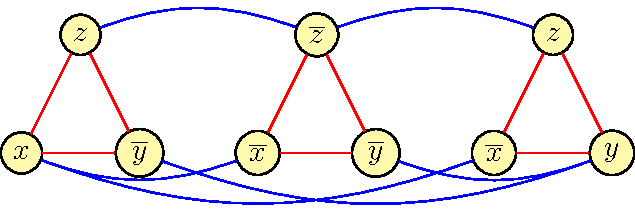
\includegraphics[width=0.9\textwidth,page=1]{gadget.pdf}
\end{center}

\end{frame}

%-------------------------------------------------------------------------
\begin{frame}{Riduzione tramite "gadget"}

La formula \textsc{3-sat} è soddisfacibile se e solo è possibile trovare un
independent set di dimensione esattamente $k$.

\bigskip
\begin{center}
\includegraphics[width=0.9\textwidth,page=2]{gadget.pdf}
\end{center}

\small
\url{https://en.wikipedia.org/wiki/Gadget\_(computer\_science)}

\end{frame}

%-------------------------------------------------------------------------
\begin{frame}{Riduzione da problema generale a problema particolare}

\BB{Ovviamente: $\textsc{3-sat} \leq_p \textsc{sat}$}

\bigskip
\BB{\EE possibile dimostrare che $\textsc{sat} \leq_p \textsc{3-sat}$?}

\pause
\smallskip
\EE possibile trasformare una formula \textsc{sat} in una formula \textsc{3-sat} usando due semplici trucchi:
\BIL
\item Se la clausola è più lunga di tre elementi, si introduce una nuova variabile e si divide la clausola in due:

\[
  (a \vee b \vee c \vee d) \equiv (a \vee b \vee z) \wedge (\overline{z} \vee c \vee d)
\]
\item Se la clausola è più corta di tre elementi, si fa "padding"

\[
  (a \vee b) \equiv (a \vee a \vee b)
\]
\EIL

\end{frame}

\begin{frame}{Transitività delle riduzioni}

\EE facile intuire che la nozione di riducibilità polinomiale gode della
proprietà transitiva

\[
  \textsc{sat} \leq_p \textsc{3-sat} \leq_p \textsc{independent-set} \leq_p \textsc{vertex-cover}
\]

\end{frame}



\section{Classi \PTIME, \PSPACE}

\begin{frame}{Classi \PTIME, \PSPACE}

\vspace{-9pt}
\begin{myboxtitle}[Algoritmo]
Dati un problema di decisione $R$ e un algoritmo $A$ (scritto in un modello di calcolo Turing-equivalente)
che lavora in tempo $f_t(n)$ e spazio $f_s(n)$, diciamo che $A$ 
risolve $R$ se $A$ restituisce $s$ su un'istanza $x$ 
se e solo se $(x,s) \in R$.
\end{myboxtitle}

\begin{myboxtitle}[Classi di complessità]
Data una qualunque funzione $f(n)$, chiamiamo:
\BIL
\item \alert{$\TIME(f(n))$} l'insieme dei problemi decisionali
 risolvibili da un algoritmo che lavora in tempo $O(f(n))$
\item \alert{$\SPACE(f(n))$} gli insiemi dei problemi 
decisionali risolvibili da un algoritmo che lavora  in spazio $O(f(n))$.
\EIL
\end{myboxtitle}

\end{frame}

\begin{frame}{Classi \PTIME, \PSPACE}

\vspace{-9pt}
\begin{myboxtitle}[Classe \PTIME]
La \alert{classe $\PTIME$} è la classe dei problemi decisionali risolvibili
in tempo polinomiale nella dimensione $n$ dell'istanza di ingresso:
\[
  \PTIME = \cup_{c=0}^{\infty} \TIME(n^c)
\]
\end{myboxtitle}

\begin{myboxtitle}[Classe $\PSPACE$]
La \alert{classe $\PSPACE$} è la classe dei problemi decisionali risolvibili
in spazio polinomiale nella dimensione $n$ dell'istanza di ingresso:
\[
  \PSPACE = \cup_{c=0}^{\infty} \SPACE(n^c)
\]
\end{myboxtitle}

\begin{myboxtitle}[Note]
$\PTIME \subseteq \PSPACE$
\end{myboxtitle}

\end{frame}

\section{Classe \NP}
%-------------------------------------------------------------------------
\begin{frame}{Classe \NP}

\vspace{-9pt}
\begin{myboxtitle}[Certificato]
Dato un problema decisionale $R$ e un'istanza di input $x$ tale
che $(x, \mathbf{true}) \in R$, un \alert{certificato} è un insieme di informazioni che permette di provare che $(x, \mathbf{true}) \in R$
\end{myboxtitle}

\begin{myboxtitle}[Esempi]
\BIL
\item \textsc{sat}: un assegnamento di verità alle variabili 
  della formula
\item \textsc{graph-coloring}: un'associazione nodo-colore $f: V \rightarrow \{ 1, \ldots, k \}$  
\item \textsc{independent-set}: un sottoinsieme di $V$ di $k$ elementi
\EIL

\medskip
Tutti questi ``certificati'' hanno dimensione polinomiale nella dimensione dell'input.
\end{myboxtitle}

\end{frame}

%-------------------------------------------------------------------------
\begin{frame}{Classe \NP}

I certificati suddetti possono essere verificati in tempo polinomiale:
\BIL
\item \textsc{sat}: si calcola il valore di verità della formula a partire dall'assegnamento di verità delle variabili in tempo $O(n)$
\item \textsc{graph-coloring}: si verifica che nodi adiacenti non abbiano lo stesso
colore in tempo $O(m+n)$
\item \textsc{independent-set}: si verifica che nodi in $V$ non abbiano nodi
adiacenti in $V$ in tempo $O(m+n)$
\EIL

\begin{myboxtitle}[Classe \NP]
L'insieme di tutti i problemi che ammettono un certificato verificabile
in tempo polinomiale.    
\end{myboxtitle}

\end{frame}



%-------------------------------------------------------------------------
\begin{frame}{Certificati non polinomiali}

\vspace{-9pt}
\begin{myboxtitle}[Quantified Boolean Formula (QBF)]
Il problema QBF è una generalizzazione del problema SAT nel quale ad ogni variabile possono essere applicati quantificatori universali e esistenziali
\end{myboxtitle}

\vspace{-3pt}
\TwoCols{
\begin{myboxtitle}[Esempio]
\[
  \forall x\  \exists y\  \exists z\  ((x  \lor z) \land y)
\]    
\end{myboxtitle}
}{
\begin{myboxtitle}[Esercizio...]
Progettate un certificato per QCB che possa essere verificato
in tempo polinomiale
\end{myboxtitle}
\pause
\BB{Si ritiene che un certificato del genere non esista}
}
\end{frame}

% %-------------------------------------------------------------------------
% \begin{frame}{Classe \NP\ -- Definizione basata su non determinismo}
%
% \vspace{-9pt}
% \begin{myboxtitle}[Classe \NP]
% \NP\ è l'insieme di problemi decisionali che possono essere risolti da
% una Macchina di Turing non deterministica in tempo polinomiale
% \end{myboxtitle}
%
% \bigskip
% \BB{In maniera mooolto informale...}
% \BIL
% \item Dato uno stato ed un elemento di input, una macchina non deterministica
% può andare in un insieme \underline{finito} di altri stati
% \item Due interpretazioni per la macchina non deterministica:
%   \BI
%   \item Macchina non deterministica che "azzecca" sempre la scelta giusta
%   \item Macchina non deterministica che si divide in un insieme finito di copie, una per scelta possibile
%   \EI
% \EIL
%
% \end{frame}
%
% %-------------------------------------------------------------------------
% \begin{frame}{Classe \NP\ -- Definizione basata su non determinismo}
%
% \vspace{-9pt}
% \begin{myboxtitle}[Esempio]
% \textsc{sat} con quattro variabili
%
% \IG{1.0}{albero10.pdf}
% \end{myboxtitle}
%
% \end{frame}

\section{Problemi \NP-Completi}

%-------------------------------------------------------------------------
\begin{frame}{Relazioni fra problemi}

\vspace{-9pt}
\begin{myboxtitle}[Lemma]
Se $R_1 \leq_p R_2$ e $R_2 \in \PTIME$, allora anche
$R_1$ è contenuto in $\PTIME$.
\end{myboxtitle}

\begin{myboxtitle}[Dimostrazione]
\BI
\item Sia $T_f(n)=O(n^{k_f})$ il tempo necessario per trasformare un input di $R_1$ in input di $R_2$ tramite una funzione $f$
\item Sia $T_2(n)=O(n^{k_2})$ il tempo necessario per risolvere $R_2$
\item Qual è la complessità per risolvere $R_1$? 
\EI
\pause\smallskip
\BI
\item La funzione $f$ può prendere un input di dimensione
$n$ e trasformarlo in un input di dimensione $O(n^{k_f})$ per $R_2$
\item Il tempo per risolvere $R_1$ sarà quindi $T_1(n) = O(n^{k_f k_2})$
\item $T_1(n)$ è polinomiale
\EI
\end{myboxtitle}
\end{frame}

%-------------------------------------------------------------------------
\begin{frame}{Definizioni}
    
\vspace{-9pt}
\begin{myboxtitle}[Problema \NP-arduo (\NP-hard)]
Un problema decisionale $R$ si dice \alert{\NP-arduo} se
ogni problema $Q \in \NP$ è riducibile
polinomialmente a $R$ ($Q \leq_p R$)
\end{myboxtitle}

\begin{myboxtitle}[Problema \NP-completo (\NP-complete)]
Un problema decisionale $R$ si dice \alert{\NP-completo} se appartiene alla
classe \NP\ ed è \NP-hard.
\end{myboxtitle}

\begin{myboxtitle}[\PTIME=\NP?]
Se un qualunque problema decisionale \NP-completo appartenesse
a \PTIME, allora risulterebbe $\PTIME=\NP$.
\end{myboxtitle}

\end{frame}

%-------------------------------------------------------------------------
\begin{frame}{\PTIME\ vs \NP}

\vspace{-6pt}
\IG{0.8}{pnp.pdf}

\tiny
\url{https://en.wikipedia.org/wiki/NP\_(complexity)\#/media/File:P\_np\_np-complete\_np-hard.svg}

\end{frame}

%-------------------------------------------------------------------------
\begin{frame}{Problemi \NP-completi: esistono?}

\vspace{-9pt}
\BB{Problema}
\BIL
\item Dimostrare che un problema è contenuto in \NP\ è semplice
\item Dimostrare che un problema è \NP-completo richiede una dimostrazione difficile, apparantemente impossibile:

\bigskip
\emph{Tutti i problemi in \NP\ sono riducibili polinomialmente a tale problema - anche i problemi che non conosciamo!}
\EIL

\bigskip
Fra i problemi visti oggi, quale potrebbe essere un buon candidato?

\end{frame}

%-------------------------------------------------------------------------
\begin{frame}{Teorema di Cook-Levin}

\vspace{-9pt}
\begin{myboxtitle}[Bibliografia]
Stephen Cook (1971). "The Complexity of Theorem Proving Procedures". Proceedings of the third annual ACM Symposium on Theory of computing (STOC). pp. 151–158. ACM.
\end{myboxtitle}

\vspace{-6pt}
\TwoColsCustom{0.65}{0.30}{
\begin{myboxtitle}[Teorema di Cook-Levin]
\textsc{sat} è \NP-completo
\end{myboxtitle}

\BIL
\item Dimostrazione complessa, basata sugli stati della macchina di Turing
\item Dimostrato nel 1973 da Leonid Levin (URSS) in maniera indipendente
\EIL
}{
\IG{1.0}{cook.jpg}
}

\tiny
\url{https://it.wikipedia.org/wiki/Stephen\_Cook\#/media/File:Prof.Cook.jpg}

\end{frame}

%-------------------------------------------------------------------------
\begin{frame}{Problemi introdotti oggi}

Partendo dalle riduzioni viste oggi e utilizzando il Teorema di Cook-Levin,
otteniamo:

\[
  \textsc{sat} \leq_p \textsc{3-sat} \leq_p \textsc{independent-set} \leq_p \textsc{vertex-cover} \leq_p \textsc{sat}
\]

\bigskip
In altre parole, \textsc{3-sat}, \textsc{independent-set}, \textsc{vertex-cover}
sono \NP-completi.

\end{frame}


%-------------------------------------------------------------------------
\begin{frame}{I 21 problemi \NP-completi di Karp}

\vspace{-9pt}
\begin{myboxtitle}[Bibliografia]
Richard Karp (1972). "Reducibility Among Combinatorial Problems". In R. Miller and J. Thatcher (eds). Proc. of Complexity of Computer Computations, pp. 85–103 (Plenum).
\end{myboxtitle}

\vspace{-9pt}
\IG{0.8}{karp-problems.pdf}

\tiny
\vspace{-24pt}
\url{http://aimsciences.org/article/doi/10.3934/naco.2018001}
\end{frame}

%-------------------------------------------------------------------------
\begin{frame}{NP Compendium}

\vspace{-12pt}
\IG{1.0}{compendium.pdf}

\tiny
\url{http://www.csc.kth.se/tcs/problemlist.html}


\end{frame}


%-------------------------------------------------------------------------
\begin{frame}{Problemi NP-Completi "Classici"}

\vspace{-9pt}
\begin{myboxtitle}[Cricca (\textsc{clique})]
Dati un grafo non orientato ed un intero $k$, esiste un sottoinsieme di almeno
$k$ nodi tutti mutuamente adiacenti?
\end{myboxtitle}

\TwoCols{
\vspace{-12pt}
\IG{0.9}{clique.pdf}
}{
\begin{myboxtitle}[Applicazioni]
\BIL
\item Bioinformatica
\item Ingegneria elettronica
\item Chimica
\EIL
\end{myboxtitle}
}

\vfill
\tiny
\url{https://en.wikipedia.org/wiki/Clique\_(graph_theory)\#/media/File:VR\_complex.svg}

\end{frame}

%-------------------------------------------------------------------------
\begin{frame}{Problemi NP-Completi "Classici"}
	
\vspace{-9pt}
\begin{myboxtitle}[Commesso viaggiatore (Traveling salesperson - \textsc{tsp})]
Date $n$ città, le distanze tra esse, ed un intero $k$, è possibile partire da
una città, attraversare ogni città esattamente una volta tornando alla città
di partenza, percorrendo una distanza non superiore a $k$?
\end{myboxtitle}

\begin{center}
\IG{0.5}{tsp.png}
\end{center}

\vfill
\tiny
\url{https://optimization.mccormick.northwestern.edu/images/e/ea/48StatesTSP.png}

\end{frame}


%-------------------------------------------------------------------------
\begin{frame}{Problemi NP-Completi "Classici"}
	
\vspace{-9pt}
\begin{myboxtitle}[Programmazione lineare $0$/$1$]
Data una matrice $A$ di elementi interi e di dimensione $m \times n$, ed un
vettore $b$ di $m$ elementi interi, esiste un vettore $x$ di $n$ elementi $0$/$1$ tale che $Ax \le b$?
\end{myboxtitle}

\begin{myboxtitle}[Esempio]
\begin{alignat*}{4}
x_1 &+ x_2 &&+ x_3 &&+ x_4 &&\ge 2\\
x_1 &- x_2 &&- x_3 &&+ x_4 &&\ge 0\\
x_1 &&&+ x_3 &&+ x_4 &&\le 1
\end{alignat*}
Il sistema è verificato per $x_1 = x_2 = 1$ ed $x_3 = x_4 = 0$.
\end{myboxtitle}

\end{frame}

%-------------------------------------------------------------------------
\begin{frame}{Problemi NP-Completi "Classici"}
	
\vspace{-9pt}
\begin{myboxtitle}[Copertura esatta di insiemi /\textsc{exact cover}]
Dato un insieme $X$ e una collezione ${\cal Y} = \{Y_1, \mldots,
Y_n\}$ di sottoinsiemi di $X$, esiste una sottocollezione ${\cal Z} \subseteq {\cal Y}$ che partizioni $X$?
\end{myboxtitle}

\begin{overprint}
\onslide<1|handout:0>
\TwoCols{
\begin{align*}
X &= \{1, 2, 3, 4, 5, 6, 7 \} \\
{\cal Y} &= \{ A, B, C, D, E, F \} \\
A &= \{1, 4, 7 \} \\
B &= \{1, 4 \} \\
C &= \{4, 5, 7 \} \\
D &= \{3, 5, 6 \} \\
E &= \{2, 3, 6, 7 \} \\
F &= \{2, 7 \}
\end{align*}
}{
}
\onslide<2|handout:1>
\TwoCols{
\begin{align*}
X &= \{1, 2, 3, 4, 5, 6, 7 \} \\
{\cal Y} &= \{ A, B, C, D, E, F \} \\
A &= \{1, 4, 7 \} \\
B &= \alert{\{1, 4 \}} \\
C &= \{4, 5, 7 \} \\
D &= \alert{\{3, 5, 6 \}} \\
E &= \{2, 3, 6, 7 \} \\
F &= \alert{\{2, 7 \}}
\end{align*}
}{
${\cal Z} = \{ B,D,F \}$
}
\end{overprint}

\end{frame}

%-------------------------------------------------------------------------
\begin{frame}{Problemi NP-Completi "Classici"}

\small
\vspace{-9pt}
\begin{myboxtitle}[Partizione (\textsc{partition})]
Dato un vettore $A$ contenente $n$ interi positivi, esiste un
sottoinsieme $S \subseteq \{1 \ldots n\}$ tale che $\sum_{i\in S} A[i] = \sum_{i \notin S} A[i]$ ?
\end{myboxtitle}

\begin{myboxtitle}[Somma di sottoinsieme (Subset sum)]
Dati un vettore $A$ contenente $n$ interi positivi ed un intero positivo $k$, \alert{esiste} un sottoinsieme $S \subseteq \ldots n\}$ tale che 
$\sum_{i \in S} a[i] = k$?
\end{myboxtitle}

\begin{myboxtitle}[Zaino (\textsc{knapsack})]
Dati un intero positivo $C$ (la capacità dello zaino) e un insieme di $n$ oggetti, tali che l'oggetto $i$ è caratterizzato da un ``profitto'' $p[i] \in \mathbf{Z}^+$ e da un peso $w[i] \in \mathbf{Z}^+$, esiste un sottoinsieme $S \subseteq \{ 1, \mldots, n \}$ tale che il peso totale $w(S) = \sum_{i \in S} w[i] \le C$ e il profitto totale $p(S) = \sum_{i \in S} p[i]$ è maggiore o uguale a $k$?
\end{myboxtitle}

\end{frame}

%-------------------------------------------------------------------------
\begin{frame}{Problemi NP-Completi "Classici"}

\vspace{-9pt}
\begin{myboxtitle}[Circuito hamiltoniano (\textsc{hamiltonian-circuit})]
Dato un grafo non orientato $G$, esiste un circuito che attraversi ogni nodo
una e una sola volta?
\end{myboxtitle}

\begin{center}
\IG{0.4}{hamiltonian-path.pdf}
\end{center}

\vfill
\tiny
\url{https://en.wikipedia.org/wiki/Hamiltonian\_path\#/media/File:Hamiltonian\_path.svg}

\end{frame}

%-------------------------------------------------------------------------
\begin{frame}{Problemi NP-completi in altre aree: Economia}
    
\BIL
\item Natural (Nash) equilibrium computation problem is NP-hard; the \textsc{clique} problem can reduced to it
  \BI
  \item T. Roughgarden. Computing equilibria: a computational complexity
perspective. Econ Theory (2010) 42:193–236
  \EI
\item \textsc{independent-set} could be used in market analysis for independent portfolio selection, where links between stocks represent correlation
  \BI
  \item V. Kalyagin, A. Koldanov, P. Koldanov, V. Zamaraev. Market Graph and Markowitz Model. Optimization in Science and Engineering: In Honor of the 60th Birthday of Panos M. Pardalos. (2014). Pages 293-306.
  \EI 
\EIL

\end{frame}

%-------------------------------------------------------------------------
\begin{frame}{La complessità si nasconde dove non te l'aspetti...}

\vspace{-15pt}
\TwoCols{
\begin{myboxtitle}[Circuito hamiltoniano]
Dato un grafo non orientato $G$, esiste un circuito che attraversi ogni \alert{nodo} una e una sola volta? 

\smallskip
\B{\NP-completo}
\end{myboxtitle}
}{
\begin{myboxtitle}[Circuito euleriano]
Dato un grafo non orientato $G$, esiste un circuito che attraversi ogni \alert{arco} una e una sola volta? 

\smallskip
\B{In \PTIME}
\end{myboxtitle}
}
\TwoCols{
\begin{myboxtitle}[Cammini massimi]
Dato un grafo $G=(V,E)$ e una funzione di peso $w$
sugli archi, trovare il cammino con peso \alert{massimo}

\smallskip
\B{\NP-completo}
\end{myboxtitle}
}{
\begin{myboxtitle}[Cammini minimi]
Dato un grafo $G=(V,E)$ e una funzione di peso $w$
sugli archi, trovare il cammino con peso \alert{minimo}

\smallskip
\B{In \PTIME}
\end{myboxtitle}
}

\end{frame}

\begin{frame}{Problemi aperti (più o meno)}

\vspace{-9pt}
\begin{myboxtitle}[Isomorfismo fra grafi]
Il problema dell'isomorfismo fra grafi richiede di determinare se due
grafi finiti sono isomorfi.
\BI
\item \B{Non sappiamo ancora.... \NP-completo? \PTIME?}
\item Dibattito ancora in corso (Ottobre 2017)
\EI
\end{myboxtitle}

\vspace{-3pt}
\TwoCols{
\begin{myboxtitle}[Primalità]
Dato un numero $n$, determinare se $n$ è primo.
\BI
\item \B{Incluso in \PTIME}
\item AKS primality test (2002-2005): $\tilde{O}(\log^{6} n)$
\EI
\end{myboxtitle}
}{
\begin{myboxtitle}[Fattorizzazione]
Dato un numero $n$, individuare i fattori primi che lo compongono.
\BI
\item \B{Sicuramente in \NP, si presume nè in \PTIME,
nè \NP-completo}
\EI
\end{myboxtitle}
}
\end{frame}


%-------------------------------------------------------------------------
\begin{frame}{Spunti di lettura}

\vspace{-9pt}
\begin{myboxtitle}[Bibliografia]
\BI
\item Jeff Erickson, Algorithm. Cap. 12, NP-Hardness\\
\url{http://jeffe.cs.illinois.edu/teaching/algorithms/}
\item Sanjeev Arora, Boaz Barak. Computational complexity: a modern approach.
Cambridge University Press, 2009\\
\url{http://theory.cs.princeton.edu/complexity/}
\EI
\end{myboxtitle}

\IG{0.6}{tsp-xkcd.png}

\vfill
\tiny
\url{https://xkcd.com/399/}

\end{frame}

\begin{OnlySlides}{Hamiltonian path and cycle}
\vspace{-12pt}
\begin{center}
\IG{0.65}{hamiltonian.png}
\end{center}
\vfill
\tiny
\url{https://xkcd.com/230/}
\end{OnlySlides}




\end{document}







